%!TEX root = ../dokumentation.tex

\chapter{Hauptteil}
\label{cha:Hauptteil}

\section{Analyse}{
\label{sec:analyse}
%In diesem Kapitel wird mit Hilfe von verschiedenen Anwendungsfällen das %Anwendungsszenario dargestellt.
\subsection{Anwendungsfälle}{
In diesem Abschnitt werden die verschiedenen Anwendungsfälle für die zu entwickelnde Grafische Oberfläche erläutert.

\subsubsection{Profil importieren}{
Der Kunde soll in der Lage sein, ein Profil in seinem Datenspeicher über die Menüführung der Workbench for Mill Plus auszuwählen. Das ausgewählte Profil soll in der Workbench geöffnet und in einem neuen Editor zur weiteren Bearbeitung angezeigt werden.
}

\subsubsection{Profil aktualisieren}{
Ist ein Profil im Editor der Workbench for Mill Plus geöffnet, soll es dem Anwender über verschiedene Methoden der Benutzerführung ermöglicht werden, die Aktualisierung des Profils zu starten. Ist das Profil zum aktuellen XML-Schema valide, soll keine Aktualisierung durchgeführt werden.
}

\subsubsection{Importiertes Profil verwenden}{
Ein importiertes Profil soll nach seinem Import in der \ac{DBWB} im Workflow des Benutzers verwendet werden können. 
}

\subsubsection{Erzeugtes Profil verwenden}{
Ein vom Aktualisierungsvorgang erzeugtes Profil soll nach seiner Erstellung in der \ac{DBWB} im Workflow des Benutzers verwendet werden können. 
}



}
\subsection{Nichtfuntionale Anforderungen}{

\subsubsection{Handhabung}{
Bei den Anwendern der \ac{DBWB} handelt es sich meist um Personen, die im Dokumentmanagement tätig sind. Von Ihnen kann kein Programmiertechnisches Expertenwissen erwartet werden. Somit ist es erforderlich, die Funktionalität zur Aktualisierung von Profilen möglichst intuitiv in den bestehenden Workflow zu integrieren.
}
\subsubsection{Wartbarkeit}{
Die einzelnen \ac{OSGi}-Bundles sowie deren Zusammenspiel muss einfach wartbar
sein, damit sie erfolgreich in das bestehende Produkt integriert werden können. Auch für Updates und zukünftige Entwicklungen ist eine gute Wartbarkeit von großer Bedeutung. Ist eine Software schlecht wartbar, lassen sich neue oder geänderte Anforderungen meist nur mit hohem Aufwand umsetzen.
}
\subsubsection{Portierbarkeit}{
Das zu entwickelnde Plug-in soll auf allen Systemen verfügbar sein, auf denen auch die Workbench for Mill Plus eingesetzt wird. Die Portierbarkeit bei modular aufgebauten Systemen hat eine große Bedeutung. Wird ihr wenig Aufmerksamkeit geschenkt, wird das entwickelte System nicht auf allen Zielplattformen das gleiche Verhalten aufweisen können.
}

\subsubsection{Konsistenz}{
Die Erweiterungen der \ac{DBWB} sollen eine Konsistenz in der Benutzerführung aufweisen. Zusätzliche Module und Plug-ins sollen nahtlos in den bestehenden Arbeitsablauf integriert werden, um die gewohnte Benutzbarkeit für den Anwender zu gewährleisten.
}


}

}

\section{Konzept}{
\label{sec:konzept}
In diesem Abschnitt wird das, dem zu entwickelnden Plug-in zugrundeliegende, Konzept erläutert.

\subsection{Grafische Einbettung}{
Die neu bereitgestellten Funktionalitäten sollen sich nahtlos in die bestehende Anwendung DocBridge Workbench for Mill integrieren. Darüber hinaus soll die grafische Einbettung den Standards der Compart AG für \ac{GUI}s genügen. Hierzu wurden die Benutzeroberfläche der \ac{DBWB} und firmeninterne Designvorlagen untersucht. Um eine hohe Benutzbarkeit zu gewährleisten werdem dem Anwender mehrere Möglichkeiten gegeben, auf die hinzugefügten Funktionalitäten zuzugreifen. Um die grafische Einbindung zu visualisieren und zu veranschaulichen wurden \glspl{Mockup}, funktionsunfähige Modelle, angefertigt.
}

\subsection{Prototyp}{
Um die in den Anforderungen geforderten Funktionalitäten herzustellen werden diese erst in einem Prototypen simuliert. Dieser beinhaltet eine Komponente zum importieren und eine Komponente zum aktualisieren von Filterprofilen. Der Prototyp konzentriert sich bei der Aktualisierungskomponente zunächst auf den Dokumenttyp \ac{AFP}. 


\subsubsection{Komponente für den Profilimport}{
Filterprofile werden in der \ac{DBWB} in einem Profile Repository verwaltet. Für gewöhnlich wird mit jeder neuen Version eines XML-Schemas ein default Profil mitgeliefert, anhand dessen Vorlage sich der Anwender ein eigenes Profil erstellen lassen kann. Das erstellte Filterprofil kann beliebig modifiziert werden. Das default Profil ist nicht zur Modifikation vorgesehen. Die Komponente liest aus dem importierten Profil die Version aus. Die Version ist in jedem Profil als Attributswert abgelegt. Anhand der Version und einem eindeutigen Identifier wird eine neue Version im Profile Repository angelegt. Das Profil wird als neues default Profil dieser Version abgelegt. Das hat den Vorteil, dass der Anwender sein importiertes Profil in der Dokumentenperspektive der \ac{DBWB} untersuchen, jedoch nicht verändern kann. Große Bedeutung kommt auch der Benutzerführung zu. In jeder der beiden Perspektiven der \ac{DBWB} ist der Import auf unterschiedliche Art und Weise zu handhaben. 


\textbf{Prozessperspektive}
 {Dem Anwender steht in dieser Perspektive eine Projektnavigation zur Verfügung. Er soll beim Import eine Auswahlmöglichkeit für das Zielprojekt haben. Importierte Profile werden in einem Unterordner 'profiles' im ausgewählten Projekt abgelegt. Anfangs war es vorgesehen, in der Prozessperspektive mehrere Filterprofile gleichzeitig importieren zu können. Während der Implementierung der Importkomponente wurde klar, dass dies der Konsistenz und Nutzerführung nicht zuträglich ist. Die Funktionalität wurde deshalb auf den Import eines einzelnen Profils beschränkt. Nach dem Import wird das Profil im Profile Repository abgelegt und in einem Editor geöffnet. Existiert im Projektunterverzeichnis 'profiles' bereits ein Profil für den entsprechenden Filtertyp soll der Nutzer die Möglichkeit haben, das alte Profil zu überschreiben oder seine Aktion abzubrechen. 
}


\textbf{Dokumentenperspektive} 
{In der Dokumentenperspektive betrachtet der Benutzer oft nur ein einzelnes Dokument, das mit Hilfe verschiedener Filter konvertiert werden kann. Deshalb ist es unnötig mehrere Profile importieren zu können. Die Komponente zur Projektnavigation ist in dieser Perspektive ebenfalls deaktiviert. Somit soll es beim Import in der Dokumentenperspektive auch nicht möglich sein, ein Projekt auszuwählen, in dem das Profil gespeichert wird. Es wird nur im Profile Repository abgelegt und in einem Editor geöffnet.


}



}

\subsubsection{Komponente zur Aktualisierung von Profilen}{
Bei der Aktualisierung von Profilen soll ein bereits vorhandenes Plug-in verwendet werden, das die Funktionalität der Konvertierung von Profilen zur Verfügung stellt. Geplant ist, dass für jeden Filtertyp ein eigenes Plug-in erstellt wird. Diese werden bei Bedarf eingebunden. Wie auch bei der Importkomponente soll sich die Aktualisierungskomponente in den bestehenden Arbeitsfluss integrieren. Ist ein Filterprofil in einem Editor ausgewählt, hat der Anwender verschiedene Möglichkeiten den Konvertierungsprozess anzustoßen. Neben einem Eintrag im Hauptmenü soll die Aktion auch über eine Toolbar und ein Kontextmenü verfügbar sein. Nach starten des Prozesses über eine der genannten Möglichkeiten wird das aktuell geöffnete Profil ermittelt. Anhand des root-Tags\footnote{Hauptelement in der Profildatei} wird der Filtertyp(z.B. \ac{AFP},\ac{PDF}) ermittelt. Anhand dieses Filtertyps wird das benötigte Konvertierungs-Plug-in festgestellt und dessen convert-Methode mit dem ausgewählten Profil als Übergabeparameter gestartet. Sobald die Konvertierung abgeschlossen ist, wird dem Anwender das originale und das generierte Profil angezeigt, um weitere Modifikationen vornehmen zu können. Zur Vergleichsanzeige der Dateien wurden folgende Ansätze untersucht.

\textbf{Erweiterung des Dokumenteneditors}{\\
Der Editor der \ac{DBWB} ermöglicht es, eine Vorschau von zu konvertierenden Dokumenten anzuzeigen. Ist beispielsweise ein Dokument im \ac{AFP}-Format gegeben und soll nach \ac{PDF} konvertiert werden, so lässt sich das Ergebnis in einem Editor bereits zur Laufzeit betrachten. Geplant war das Überschreiben dieses Editors mit einem Standard XML-Editor. Dieser Ansatz musste verworfen werden, da dies im konzeptionellen Widerspruch zum Dokumenteneditor stand.
}

\textbf{Erstellen eines spezialisierten Editors}{\\
Der nächste Ansatz war es, einen Editor speziell zum Vergleich von zwei Filterprofildateien zu entwickeln. Ein EditorPart soll zwei weitere EditorParts enthalten, in denen das originale und das konvertierte Profil angezeigt werden. Eclipse \ac{RCP} sieht jedoch vor, dass ein Editor in Beziehung zu genau einer Datei steht. Deshalb musste dieser Ansatz ebenfalls verworfen werden. 
}

\textbf{Nutzung von CompareUI\footnote{Java \ac{API}
 um Vergleich von Objekten}}{\\
 Die Java \ac{API} CompareUI bietet einen Einstiegspunkt, um konfigurierbare Vergleichsoperationen auf beliebige Ressourcen durchzuführen. Das Ergebnis eines Vergleichs kann in einem speziellen Vergleichseditor geöffnet werden. Dieser Editor ermöglicht das dynamische Vergleichen einzelner Elemente von Dokumenten, was besonders am Beispiel von \ac{XML} oder \ac{HTML} ersichtlich wird. Auch das Eclipse Plug-in eGit\footnote{Plug-in zur grafischen Bedienung der Versionierungssoftware Git} nutzt die CompareUI, um Dateien in der Versionierungshistorie zu vergleichen. Da die Vorteile dieser Technologie nicht von der Hand zu weisen sind, wird dieser Ansatz zur Entwicklung zur Darstellung des Ergebnisses des Konvertierungs-Plug-ins gewählt.

\begin{figure}[htbp] 
  \centering
     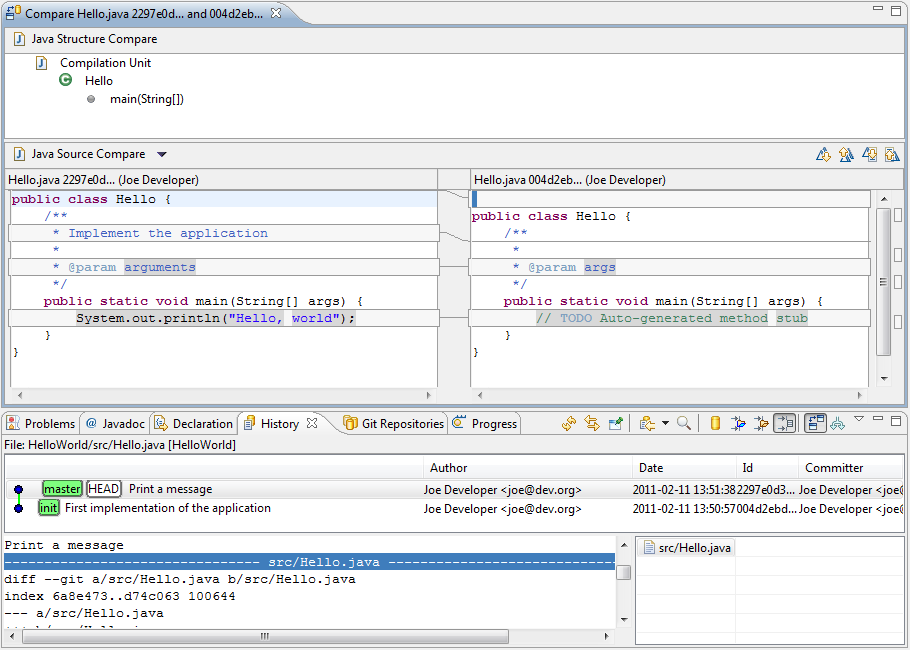
\includegraphics[height=.7\textwidth]{egit_compare.png}
  \caption{Verwendung der API CompareUI am Beispiel von eGit}
  \label{fig:egit_compare}
\end{figure}

}



}

}






\subsection{Design der Bundles}{
In der Softwareentwicklung ist die Unterteilung der Software in kleinere Einheiten vorteilhaft, da dies den Test, die Wartung und die Entwicklung allgemein vereinfacht.




}

\section{Implementierung}{
\label{sec:implementierung}
Dieser Abschnitt beschreibt die Implementierung der Komponenten für den Profilimport und die Aktualisierung der Filterprofile.

\subsection{Entwicklungsumgebung}{
Die Implementierung der Bundles erfolgt in der \ac{IDE} Eclipse\footnote{Version Kepler}. Da \ac{RCP} auf dem Eclipse-Framework basiert, liegt die Wahl dieser \ac{IDE} nahe. Für das Konfigurationsmanagement wird das Build-Management-Tool Apache Maven 2 verwendet. Als Laufzeitumgebung wird die \ac{JRE}6 verwenden, da diese auch bei den bestehenden Bundles im Entwicklungsumfeld zum Einsatz kommt.
}




\subsection{Komponente für den Profilimport}{
\label{sec:impl_import}

\subsubsection{Extensions}{
Unter Verwendung des Extension-Point-Mechanismus von Eclipse \ac{RCP} wurden in der Plugin.xml des Bundles verschiedene Extensions angelegt.
\\
\textbf{Grafische Steuerelemente}\\
Für das ergänzen der Benutzeroberfläche der \ac {DBWB} wird der Extension-Point org.eclipse.ui.menu verwendet. Sowohl in der Toolbar der \ac{DBWB} als auch in ihrer Menüleiste werden Buttons bzw Menüeinträge hinzugefügt. Das aktivieren eines solchen Menüeintrags oder Buttons startet den in "REF" beschriebenen Handler. Listing \ref{lst:extension} zeigt den Einsatz einer Extension, um eine neue Menükontribution anzulegen.

\textbf{Handler}{
\\
Neben den Extensions für die grafischen Steuerelemente wird eine Extension am Extension-Point org.eclipse.ui.handlers registriert. Dieser ImportHandler ist aktiv, falls in der Prozessperspektive ein Projekt selektiert ist, oder der Nutzer sich in der Dokumentenperspektive befindet.("REF") 
}

 \begin{lstlisting}[caption={Toolbar Extension},label=lst:extension]
 
 /**
  * This is a doc comment.
  */
 // extension beispiel code
 \end{lstlisting}


}

\subsubsection{Implementierte Klassen}{

}







}

\subsection{Komponente zur Aktualisierung von Profilen}{
\label{sec:impl_aktualisieren}
Da der Aufgabenzeitraum für die Analyse, Konzeption und Implementierung beider Komponenten zu knapp bemessen war, konnte die Aktualisierungskomponente nicht vollständig implementiert werden. Es existiert jedoch ein Prototyp, der mit der Technologie CompareUI(Abbildung \ref{fig:egit_compare}), die bereits im \nameref{sec:konzept} erwähnt wird, realisiert wurde. Es wurde eine Standalone Eclipse \ac{RCP}-Anwendung implementiert, die über die Funktionalität verfügt, einen Vergleichseditor mit zwei Profilen zu öffnen. Da bereits ein detailliertes Konzept besteht, dürfte die Implementierung dieser Komponente nicht allzu Zeitaufwendig sein. Vor allem, da Sie sich nicht in großem Maß von der Programmierung der \nameref{sec:impl_import} unterscheidet.    


}



\subsubsection{Verwendete Bibliotheken}{

}



}


\section{Ergebnisse}{
\label{sec:ergebnisse}


}




}

